\documentclass[times, utf8, diplomski]{fer}
\usepackage{booktabs}
\usepackage{algorithmic}
\usepackage{algorithm}
\usepackage{listings}
\usepackage{longtable}
\usepackage{graphicx}
\usepackage{array}
\usepackage{enumitem}
\usepackage{multirow}
\usepackage{amsmath}

\newcolumntype{P}[1]{>{\centering\arraybackslash}p{#1}}
\newcolumntype{M}[1]{>{\centering\arraybackslash}m{#1}}

\begin{document}

% TODO: Navedite broj rada.
\thesisnumber{1720}

% TODO: Navedite naslov rada.
\title{Projektiranje sustava praćenja trajektorije bespilotne letjelice u sustavu globalne vizije}

% TODO: Navedite vaše ime i prezime.
\author{Luka Galović}

\maketitle

% Ispis stranice s napomenom o umetanju izvornika rada. Uklonite naredbu \izvornik ako želite izbaciti tu stranicu.
\izvornik

% Dodavanje zahvale ili prazne stranice. Ako ne želite dodati zahvalu, naredbu ostavite radi prazne stranice.
\zahvala{Svima koji žele naučiti koristiti \LaTeX{}.}

\tableofcontents
% Tu možete staviti popis slika i tablica

\chapter{Uvod}
Ulaskom u novo stoljeće svjedočimo nastavku razvoja, usavršavanja i stvaranja novih tehnologija koja su pomoć u različitim ljudskim aktivnostima. Iako pojam bespilotnih letjelica postoji već dugi niz godina, one su tek u bliskoj prošlosti postale pojam svakodnevnice. Dugi niz godina bespilotne letjelice su se koristile, nažalost, samo u vojnim svrhama zbog čega su stradavali i nedužni civili zbog čega se njihov razvoj držao u tajnosti. Samo saznanje da se koriste u vojsci upućuje na to da je puno vremena i novaca uloženo u njihov razvoj, preciznost, nosivost te izdržljivost.\\
Danas se uz nagli tred upoznavanja s tehnologijama bespilotnih letjelica, kao i digitalnih zapisa i pohranjivanja memorije svakodnevnih događaja namjena korištenja promijenila te su uvedeni novi pojmovi poput \glqq dronovi\grqq --- suvremena riječ koja zapravo opisuje nekoliko vrsta bespilotnih letjelica. Glavna područja njihovih korištenja su: javna sigurnost, zabava, nadzor i inspekcija, informacije, znanost o Zemlji.\\
Korištenje  bespilotnih letjelica, naročito u civilne svrhe, bilježi eksponencijalan rast, kako u pogledu njihovog broja, veličine i težine, tako i u pogledu sve brojnijih mogućnosti njihove primjene \citep{EUR-Lex}. Cilj je razviti jeftinije i sposobnije bespilotne letjelice. U skoroj budućnosti tehnologija će se usavršiti pa će manje letjelice moći prenositi sve veću opremu, tako npr.~poštanski paketi će se dostavljati pomoću letjelica.\\
Motiv izrade ovog rada leži u širokoj primjeni (kako u različitim granama industrije i istraživanja tako i za zabavu). Cilj ovog rada je shvatiti rad bespilotne letjelice te izrada sustava za slijeđenje željene trajektorije. Izazov je kretati se zadanom trajektorijom znajući da postoje razne vanjske smetnje koje utjeću na upravljanje. U teorijskom dijelu će se opisati razvoj, svrha odnosno tipovi bespilotnih letjelica, dok će se detaljnije razraditi njezin model te odrediti matematički model prikladan za sintezu sustava upravljanja. Projektirat će se regulator za slijeđenje reference, uz pretpostavku raspoloživosti informacije o trenutnoj poziciji te orijentaciji. Provjera projektiranog sustava je u simulaciji odnosno eksperimentalno u laboratorijskim uvjetima.

\chapter{Razrada}
\section{Bespilotne letjelice}
Bespilotne letjelice (UAV\footnote{UAV \engl{Unmanned Aerial Vehicle} – opći je pojam koji označava zapravo sve vrste bespilotnih letjelica koje se kolokvijalno najčešće nazivaju dronovima. Pod tim se obično spominju dvije vrste letjelica kojima ne trebaju ljudski piloti, prve su tzv. kvadrikopteri \engl{quadcopter}, letjelice s četiri elise pomoću kojih dron može lebdjeti na mjestu i kretati se u raznim smjerovima. Drugi tip bespilotnih letjelica su izgleda projektila ili zrakoplova kojim se upravlja iz baze i povezani su uglavnom s vojnim operacijama.}) su, najjednostavnije rečeno, letjelice koje su sposobne izvršiti kontinuirani let bez prisutnosti pilota \citep{UAV}. Postoje razni oblici i veličine, no najčešće su dizajnirane za točno specifične uloge.\\
U nastavku bit će navedeni kratak pregled bespilotnih letjelica kroz povijest, njihova definicija, vrste te primjena.\\
Današnji dronovi su opremljeni raznim senzorima (akcelometri, giroskopi, kamere) koji olakšavaju njihovo upravljanje i točnost pozicioniranja u prostoru.
%Definiranjem pojma bespilotnih letjelica nailazi se na bogat izbor objašnjenja jer imaju široku primjenu. \\

\subsection{Pregled povijesti}
Početak razvoja bespilotnih letjelica je usko vezan s razvojem svih zrakoplova. Povijest seže u prošlo stoljeće kada su Kinezi puštali papirnate zmajeve prema nebu ili letjeli u balonima na vrućem zraku, iako bi se moglo reći da je prva bespilotna letjelica kamen koji je bacio špiljski čovjek u pretpovijesno doba. Ove \glqq letjelice\grqq imaju malo ili nimalo kontrole. U suvremenom dobu, bespilotnim letjelicama se nazivaju sve letjelice koje su imale autonomno ili daljinsko upravljanje. Razvojem tehnologija i moderniziranjem nazivi i opisi ovih letjelica se mijenjaju poput ratnih torpeda, bespilotnih vozila, daljinski upravljača, autonomna kontrola, dron itd.\\
U ranim godinama zrakoplostva, sama ideja da zrakoplov leti bez ljudskog faktora imala je veliku prednost u tome što je na taj način u potpunosti uklonila rizik za život. No pojavio se veliki nedostatak kod mogućnosti upravljanja takvim letjelicama, odnosno postojala su određena ograničenja. Tako su bespilotne letjelice bile opisivane kao 3D \engl{dangarous, dirty, dull} --- opasne, prljave i glupe. Opasne su jer njima netko može srušiti zrakoplov i dovesti u opasnost pilota i ostale putnike, zatim prljave su jer se kreću na mjestima koja su izložena kemijskom, biološkim ili radiološkim opasnostima, te glupe jer je potrebno njima upravljati nekoliko sati što postaje stresno i nepoželjno \citep{unmannedAircraftSystem}. Danas se upotreba i korištenje znatno promijenilo te su one postale popularan izvor zabave, uz svrhu i na nekim drugim područjima.\\
Bespilotne letjelice kao takve, bile su prepoznatljive i prije Prvog svjetskog rata. Tome su  doprinijeli ljudi koji su ih već tad koristili za područje istraživanja i slično. Konkretnije, 1883.  godine  Douglas  Archibald, po  nacionalnosti Englez,  na liniju  „zmaja“  stavio  je anemometar  te  je  mjerio  brzinu  vjetra  na  raznim  nadmorskim  visinama. Nekoliko  godina kasnije, na „zmaj“ je priključio kamere te je na taj način proizveo prvo izviđanje putem letjelice. Nadalje, William Eddy snimio je tisuće fotografija koristeći „zmaj“ s kamerama tijekom rata što se može smatrati prvim korištenjem bespilotnih letjelica za vrijeme ratne borbe\citep{UAVSystems}.\\
Veliki razvoj bespilotnih letjelica vidljiv je u vojne svrhe. Charles  Kettering  razvio  je  bespilotnu  letjelicu  s  dva  krila, tzv.~dvokrilac za tadašnju vojsku (\emph{Army Signal Corps}). Tri godine razvoja dovele su do letjelice nazvane „\emph{Kettering Aerial Torpedo}", odnosno „\emph{Kettering Bug}“ ili samo „\emph{Bug}“. Letjelica je mogla letjeti približno 40 do 55 m/h te nositi oko 80 kg teškog eksploziva. Bila usmjerena prema cilju sa svojim postavkama i imala  je  odvojiva  krila  koja  bi  se ispustila u  trenutku kada  bi  letjelica  bila iznad  mete dopuštajući trupu aviona da padne na tlo kao bomba.  Također 1917.~, Lawrence Sperry je razvio UAV, sličan kao od Katteringa. Letjelica je imala naziv \emph{Sperry - Curtis Aerial Torpedo}, a bila je namjena za mornaricu. Imala nekoliko uspješnih letova, no nikad se nije koristila u ratu. Tvrtka pod nazivo \emph{Radioplane Company} je izradila tisuće ciljnih dronova \engl{target drones} za vrijeme drugog svjetskog rata. Nijemci su u kasnijim godinama drugog svjetskog rata koristili smrtonosne bespilotne letjelice V-1 i V-2. Tek su se u vrijeme Vijetnamskog rata bespilotne letjelice uspješno koristile kao sredstva za nadziranje odnosno izviđanje. (Fahlstrom, Gleason, 2012., str. 4). Značajnu ulogu bespilotne letjelice imale su i u ratovima u Bosni i Afganistanu.\\
Nadalje, tijekom zadnjih nekoliko godina ovakve letjelice su se sve više razvijale i modernizirale te se njihova svrha i način korištenja promijenio. Ovakav razvoj doveo je do pitanja hoće li bespilotne letjelice, odnosno sustavi bespilotnih letjelica, zamijeniti zrakoplove i letjelice za koje je potreban ljudski faktor. Postoje u potpunosti automatizirane letjelice čiji je kontrolni sustav neovisan o vanjskim signalima, a i one koje sadržavaju mogućnosti ručnog upravljanja  od  strane  pilota.  Teoretski,  potpuno  automatizirane  letjelice  mogu  letjeti  bez utjecaja ili ometanja od strane bilo kakvog signala, no njihov nedostatak je taj što mogu biti kontrolirane od strane računala. Na taj način je omogućeno manipuliranje sustavom te unatoč jakoj enkripciji,  još  uvijek  postoji  sigurnosni  rizik  i  opasnost.  Upravo  zbog  toga  te  same kontrole  i  sigurnosti  zrakoplova, i njihovih putnika, odgovornost koju pruža ljudski faktor u zrakoplovstvu, spriječit će da bespilotne letjelice postanu prioritet ili da u potpunosti zamijene normalne letjelice \citep{UAVSystems}.\\
Danas se vojna upotreba bespilotnih letjelica može 
podijeliti na tri područja, to su pomorska, kopnena i zračna upotreba, dok se u civilne  svrhe  može  upotrijebiti  u  različitim  područjima ljudskih  aktivnosti  kao  npr.  u  geodeziji  tj. fotogrametriji,   poljoprivredi,   industrijskoj proizvodnji,  civilnoj  zaštiti,  upravljanju katastrofama,  zaštiti  okoliša,  nadzorom policijskog    djelovanja,    obavještajnim službama,   novinarstvom,   komercijalnim djelatnostima, razonodom itd. Također  je  sve  veća  uporaba  bespilotnih letjelica za inspekciju   nepristupačnih dijelova  u industrijskim  objektima  kao  što su: brane, dalekovodi, visoki dimnjaci, cjevovodi, mostovi i dr. Isto tako sve popularniji i mali modeli namijenjeni za razonodu.

\subsection{Definicija bespilotnih letjelica}
Za pojam bespilotnih letjelica koristi se engleski službeni naziv „Unmanned Aerial Vehicle“,  dok  se  zadnjih  nekoliko  godina  pojavio  pojam  UAS  \engl{Unmanned  Aerial System}. Time se htjelo naglasiti činjenica da su to složeni sustavi koji uključuju i postaje na zemlji te mnoge druge elemente, a ne samo letjelice koje lete zrakom. Međutim, pojam UAS nije punokorišten za razliku od pojma UAV koji je postao dio modernog leksikona 
(The UAV, n.d.).\\
Bespilotne letjelice lete bez ljudskog pilota, umjesto toga kontrolira ih operator na tlu. Svrha bespilotnih letjelica, odnosno u ovom slučaju se govori o sustavu bespilotnih letjelica (UAS),  tj.  dronova, je  dostava poruke,  paketa  ili  samo  skupljanje  podataka. Kao najvažnija svrha sustava je upravo prikupljanje podataka. Letjelice poput dronova, a i neke druge, mogu prodrijeti  u  područja  i  lokacije  do  kojih  čovjek  ne  može  bez  određene  opasnosti  i  rizika. Ponekad, podaci mogu biti presudni za određene operacije ili aktivnosti. Također, navodi se da je jedna od karakteristika ovakvih sustava to što ih se može ponovno koristiti, odnosno to što se vraćaju (Unmanned Aerial Vehicle Systems Association, 2016).

\subsection{Prednosti i nedostaci}
Postoji nekoliko prednosti i nedostataka koje pružaju bespilotne letjelice. Prednost u odnosu na letjelice s pilotom je upravo u tome, što bespilotne letjelice ne trebaju imati pilota 
koji fizički  mora  biti  unutar  letjelice  u
pravljati  njome.  Nadalje, jedna od prednosti je ta što mogu doći na nedohvatljiva područja za ljude, a obavljaju precizno i kvalitetno snimanje terena. Mogu ostati u zraku i do 30 sati (Advantages of UAS, 2016). Samim time, bespilotna letjelica predstavlja sigurno okruženje te se može kretati dosta velikom brzinom. Ukoliko dođe do pada letjelice, nema štete od stradanja pilota, a uz to mogu letjeti u zonama u kojima postoje velike opasnosti i to na duže vrijeme (Soffar, 2016). \\
Prednosti koje dronovi pružaju su njihova niska cijena te je održavanje puno jeftinije od običnih letjelica i zrakoplova. Uz to, dronovi mogu letjeti na niskim nadmorskim visinama za razliku od zrakoplova, a također mogu letjeti nekoliko sati bez prestanka. Njihove sposobnosti snimanja, nadziranja, nadgledavanja, izviđanja jedne su od velikih prednosti kao i laka i brza implementacija sustava (Phil for Humanity, 2016).\\
S  druge  strane,  postoje  i  neki  nedostaci  bespilotnih  letjelica  i  dronova. Bespilotne letjelice su u odnosu na dronove, skupe za proizvodnju,dok se veliki troškovi mogu pojaviti i ljudskom greškom kod letjelica s daljinskim upravljanjem te to može uzrokovati njen pad. Također, može se dogoditi i to da se letjelica izgubi što također donosi velike troškove. Kvarovi na računalu isto mogu uzrokovati štete na bespilotnim letjelicama, naročito kada se one koriste za vojne napade što može rezultirati ubijanjem civila i uništenjem  civilne  imovine (Soffar, 2016). \\
Unatoč tome, vojska i dalje koristi dronove i  bespilotne letjelice jer vjeruju u njihove prednosti, a nisu svjesni nedostataka. Nedostaci dronova su ti da oni ne mogu komunicirati s civilima, odnosno u slučaju vojnog napada te potrebe za evakuacijom nekog područja. Loše programirani dronovi mogu izazvati velike štete, a kao takvi mogu biti preuzeti od strane neprijatelja što dovodi u pitanje sigurnost takvih sustava. 


 

\subsection{Vrste}
Prema Fahlstorm  i  Gleason  (2012.) postoje  3  vrste  letjelica  bez  pilota,  isključujući 
projektile: \begin{itemize}
\item Bespilotne letjelice \engl{Unmanned Aerial Vehicle - UAV}
\item Letjelice na daljinsko upravljanje \engl{ Remotely Piloted Vehicle - RPV}
\item Dronovi \engl{Drones}
\item Oblik muhe \engl{insect fly shaped drone}
\end{itemize}
U današnje doba, najčešći pojam koji se javlja za opisivanje bespilotnih letjelica je dron. Razlika između drona i bespilotne letjelice (UAV) je u stupnjuautomatizacije, jer dronov let ovisi o unaprijed programiranom ponašanju, a kod UAV postoji daljinsko upravljanje od strane pilota  u  kontrolnoj  stanici (UAV  Insider,  2013). U ovom radu bit će naglasak na treću vrstu bespilotnih letjelica koje se sve više i više danas koriste, a to su dronovi. 

\subsubsection{UAV}
Kao što je već spomenuto, bespilotna letjelica je letjelica ili zrakoplov bez pilota. Njome se može upravljati na daljinski, odnosno od strane osoba koja to čini u kontrolnoj stanici. S druge strane, može letjeti samostalno na temelju unaprijed programiranih planova leta ili više složenih dinamičkih sustava za automatizaciju. Takve letjelice se koriste za mnoge svrhe i misije, najčešće u slučaju izviđanja, no ponekad imaju i napadačke uloge. Sposobnosti koje posjeduje su te što može biti kontrolirala, ima održiv horizontalni let i pokreće se pomoću mlaznog ili klipnog motora. Postoji nekoliko tipova ovakvih letjelica, a klasificirane su prema svrsi koju obavljaju (The UAV, n.d.):
\begin{itemize}
\item Za pronalaženje ciljeva i meta --- pronalazi zemaljske i zračne neprijateljske mete 
\item Izviđačke --- omogućuje pronalazak ratnih polja
\item Za borbu --- ima napadačku sposobnost za visoko rizične misije
\item Za istraživanje i razvoj --- koristi se za daljnji razvoj tehnologije
\item U građanske i trgovačke svrhe --- posebno dizajniran za državne i komercijalne svrhe
\end{itemize}
Neke  od  bespilotnih  letjelica  su:  Altair,  Global  Hawk,  X47-A, Prowler II, X45-A UCAV, Fire Scout, Predator A i Predator B, ER/MP UAS, I-GNAT, Mariner, Army I-GNAT ER i drugi.
\begin{figure}[htb]
\centering

\includegraphics[width=5cm]{img/fer_logo.jpg}
\caption{Bespilotna letjelica\protect\footnotemark}
\label{fig:bespilotna letjelica}
\end{figure}
\footnotetext{www.sadasfasdfasfas}

\subsubsection{RPV}
RPV su letjelice na daljinsko upravljanje \engl{ Remotely Piloted Vehicle}. Takve male letjelice  su  najviše  korištene  za  terenski  rad  vezan  uz  okoliš. Prema  tome,  njihov  raspon korištenja kreće se od šumarstva, morskih istraživanja, promatranja biljnih i životinjskih svijeta, dobivanja uzoraka o biološkim stvarima iz zraka i slično. Prednosti takvih letjelica su u tome što je pilot siguran, odnosno nije fizički prisutan. Zatim, brzo prikupljanje podataka, niska cijena te relativno kratko vrijeme odaziva i dobivanja odgovora na zahtjeve. No s druge strane, postoje i neka ograničenja prilikom takvih letjelica, a to su niska stabilnost kao fotografske platforme, kratko vrijeme leta, malobrojnost senzora, teškoće kod navigacijskog sustava itd. \\
Daljnji razvoj i korištenje letjelica na daljinsko upravljanje je upravo za potrebe snimanja stana okoliša. Osim otkrivanja i procjene okoliša, potreban je i daljnji fokus na poboljšanje slike te omogućiti ugradnju više senzora za razna mjerenja \citep{Hardin}.

\subsubsection{Dronovi}
Vrsta bespilotnih letjelica, poznatiji kao dronovi su zračni bespilotni sustavi koji mogu biti kratkog ili dugog dometa, a koriste se za vojne ili civilne svrhe. Najčešća oprema koju dron sadržava je kamera, a neki mogu biti naoružani projektilima. 
\begin{figure}[htb]
\centering

\includegraphics[width=5cm]{img/fer_logo.jpg}
\caption{Bespilotna letjelica\protect\footnotemark}
\label{fig:dron}
\end{figure}
\footnotetext{www.sadasfasdfasfaass}
Na  slici~\ref{fig:dron}  nalazi  se  slika 
drona. Današnja najvažnija primjena dronova je stvaranje mapa, odnosno snimaka iz zraka. Dronovi su  vrlo dobri u izradi karata, daleko više od drugih tehnologija za istu primjenu. Nadalje, odlični su u fotografiranju i računalnoj  obradi  tih  fotografija \citep[str.~10]{Drones}. Većina dronova koriste razne senzore kako  bi  napravili  procjenu  stanja,  odnosno  koriste  MEMS\footnote{\engl{Microelectromechanical}} čipove  za  mjerenje  ubrzanja  i rotacije. Neki od njih nose sustav za mjerenje udaljenosti od tla te također mogu imati barometre za  mjerenje  tlaka  zraka.  Uz  to,  dronovi  mogu  imati  na  sebi senzore  za  prijenos  topline  pa  i manetometre za mjerenje zemljinog magnetnog polja. No najveća većina njih posjeduje GPS senzore jer MEMS senzori koji se koriste na takvim jeftinim letjelicama nisu dovoljni precizni. No, GPS ne može ažurirati svoju poziciju dovoljno često te ima svoje oscilacije pa je najbolja kombinacija  upravo  spomenutih  senzora \citep[str.~13]{Drones}.\\
Nadalje, na slici~\ref{fig:konfiguracijaDrona} nalazi se primjer jedne od konfiguracija drona s više motora. Sastoji  se  od  spomenutih  motora  i  propelera,  kontrolera  za  let,  GPS  senzora,  baterije, elektroničkog kontrolera za brzinu, prijemnika, ploče za napajanje i telemetrijskog modula. 
\begin{figure}[htb]
\centering

\includegraphics[width=5cm]{img/fer_logo.jpg}
\caption{Bespilotna letjelica\protect\footnotemark}
\label{fig:konfiguracijaDrona}
\end{figure}
\footnotetext{http://drones.newamerica.org/primer/DronesAndAerialObservation.pdf
}

\subsection{Zakonska regulativa\citep{Ekscentar}} 
Zabilježavanjem nezakonitih upotreba bespilotnih letjelica kojima su ugrožavani ljudski životi i koji nisu u skladu s određenim zakonima (zakon o zaštiti osobnih podataka), kako bi se ograničila i osigurala upotreba bespilotnih letjelica potrebna je zakonska regulativa o toj temi. S obzirom na to da korištenje dronova, povećanjem njihovog broja, prvenstveno za zabavu postaje veoma popularno i u Republici Hrvatskoj, javlja se potreba za razmotranje i zakonske regulative\footnote{Zakon o dronovima: \url{http://www.dronovi.hr/zakon-o-dronovima.html}}.  Letjelice  se  mogu  vrlo  lako  nabaviti  ili  izraditi  te  postoji mogućnost preplavljenosti zračnog prostora. Zbog toga je potrebno registrirati svaku letjelicu i regulirati njezinu uporabu. Tako je prema Pravilniku o sustavima bespilotnih zrakoplova utvrđeno, osim općih odrednica o klasama područja letenja i letačkih operacija te veličine samih bespilotnih letjelica, to da se let bespilotnim letjelicama smije odvijati samo danju. Nadalje, potrebno je osigurati sigurnu udaljenost letjelice od ljudi, objekata, vozila, cesta, dalekovoda i drugo. Rukovoditelje bespilotne letjelice mora od nje biti udaljen do 500 metara te mu ona uvijek mora biti unutar vidnog polja. Što se tiče zrakoplova, let  drona  mora  biti  udaljen  najmanje  3  kilometara  od  aerodroma.  Dakako,  zabranjeno  je izbacivanje bilo kakvih predmeta iz letjelice. \\
No kako se dronovi najčešće koriste za snimanja iz zraka, postoje zakoni koji se moraju poštovati i za to. Dakle, navodi se da snimati iz zraka smiju pravne i fizičke osobe koje su za to pravodobno registrirane. Zatim je potrebno podnijeti zahtjev za izdavanje odobrenja za snimanje s dostavom  raznih  podataka (geodetsko snimanje koje se predaje Državnoj geodetskoj upravi):
\begin{itemize}
\item podatke o naručitelju snimanja
\item podatke o izvršitelju snimanja i dokaz o registriranoj djelatnosti iz zraka izvršitelja snimanja (potrebno priložiti kopiju registracije pri Trgovačkom sudu)
\item podatke o izvršitelju razvijanja
\item podatke o vremenu snimanja
\item svrhu snimanja
\item popis objekata, skicu ili kartu s označenim područjem snimanja
\item podatke o vrsti i mjerilu snimanja, kameri, žarišnoj daljini objektiva, filmu ili obliku zapisa (analogni/digitalni)
\item način čuvanja izvornih podataka snimanja.
\end{itemize}.
Tek nakon dobivanja odobrenja može se pristupiti snimanju te kasnije i razvijanju zračnih snimaka i pri tome je dužna najkasnije u roku od 8 dana od dana snimanja dostaviti zračne snimke na pregled Državnoj geodetskoj upravi (Zakon o obrani, NN 33/02), dok je za bilo kakvo umnožavanje, objavljivanje ili iznošenje snimaka iz Hrvatske potrebno  pribaviti  odobrenje  uz  suglasnost  ministarstva (Ministarstvo  pomorstva,  prometa  i infrastrukture, 2015).\\
Prilikom snimanja iz zraka pojedinih vojnih, telekomunikacijskih, energetskih i industrijskih objekata, područja nacionalnih parkova i parkova prirode te drugih zaštićenih dijelova prirode, također je potrebno priložiti i mišljenje korisnika objekta, odnosno ustanove koja upravlja zaštićenim dijelom prirode (Uredba o snimanju iz zraka, NN 116/03). Digitalni oblik obrasca Zahtjeva za izdavanje odobrenja za razvijanje zračnih snimaka može se pronaći na službenim internetskim stranicama Državne geodetske uprave, a uz obrazac je potrebno priložiti dokaz o registriranoj djelatnosti za snimanje iz zraka, dok je za letjelicu potrebno priložiti kopiju Certifikata za obavljanje radova iz zraka s Operativnim specifikacijama koju izdaje Agencija za civilno zrakoplovstvo.\\

\subsection{Primjena i rasprostranjenost}
Kako bespilotne  letjelice  postaju  manje,  jeftinije  i  jednostavnije za  upravljanje,  a regulatorne izmjene, naročito u SAD-u, smanjuju prepreke za nove korisnike, letjelica je sve više. 
Prema izvješću tvrtke PwC (Price Waterhouse Coopers) “Clarity from above“ može se govoriti o globalnoj tržišnoj vrijednosti rješenja baziranim na bespilotnim letjelicama višoj od 127,3 milijardi dolara.
Očekuje se da će povećanjem broja letjelica smanjiti nesreće na radu, 
poput pada zaposlenika s krova tijekom inspekcija zgrada, a time i gubici zbog kompenzacija 
radnicima. 
Bespilotne letjelice bi u budućnosti mogle riješiti niz problema i smanjiti troškove i u nizu drugih industrija, u zemljama u razvoju i slučajevima prirodnih katastrofa. (Allianz, 2017.)
Kao što je navedeno ranije, postoji podjela bespilotnih letjelica (UAV) prema njihovoj svrsi. Tako  su  najprije  bile  namijenjene za korištenje u vojne svrhe, no danas je njihova primjena puno veća (Stombaugh, Smith, Thamann, n.d.). Ostala područja u kojima se danas koriste su:\begin{itemize}
\item geodezija --- projektiranje, rudarstvo, geologija, šumarstvo
\item poljoprivreda
\item kotrola i nadzor nad kritičnom infrastrukturom
\item sigurnost i okoliš
\item praćenje i nadzor okoliša
\item potraga i spašavanje
\item sigurnost
\item dostava
\end{itemize}
U  vojne  svrhe bespilotne  letjelice  se  koriste  za  sigurnosni  nadzor  i  kontrolu  vojnih područja, za zračne izvidnice, otkrivanje kemijskih, bioloških, radioloških i nuklearnih uvjeta na nekom terenu, zatim za telekomunikacijski promet, za potragu i spašavanje i dr. Što se tiče terenskog  pretraživanja  i  spašavanja,  vrše  nadgledanje  i  obilježavaju  točke  na  kojima  je potrebna intervencija i slično. Nadalje, bespilotne letjelice  su  korisne  i  u  telekomunikacijske svrhe, a čak mogu i detektirati lansiranje nekog projektila (Military UAS Application, 2016).\\
U poljoprivredi se pomoću dronova ili drugih vrsta bespilotnih letjelice za tu svrhu, nastoji povećati produktivnost i efikasnost  proizvodnje.  Dronovi  se  mogu  koristiti  za  nadzor usjeva,  provjeru  uvjeta  na  zemljištu  da  bi  se  tako  ostvario  ekološki  održiv  način  rada,  tj. racionalnije koristila voda, upotrebljavali pesticidi pa i pametnije koristili strojevi. U geodeziji, bespilotne letjelice mogu snimati teren te se na temelju toga može izraditi 3D prikaz, razni digitalni modeli terena i površine itd. Dronovi su korisni jer mogu doći do nepristupačnih terena i područja te obaviti potrebno snimanje  i mjerenje.  Nadalje,  bespilotne letjelice  mogu  biti korisne kod mjerenja infrastrukture i vrše točan, brz i pouzdan nadzor nad objektima zajedno sa preciznim i učinkovitim ugrađenim kamerama(Geo-Tron, 2015)\\
Praćenje  okoliša,  snimanje  šuma,  procjena  kvalitete  zraka,  kontrola   i nadzor nad kritičnom infrastrukturom (npr.~odlagališta  i otpadne  vode)  te  mnoge  druge  mogućnosti  vezane  uz  okoliš  karakteristične  su  dronove. Prednost je u tome što takva snimanja i prikupljanja podataka nisu skupa te ne postoje veliki financijski troškovi, a ne ovise niti o vremenskim uvjetima.\\
Također, bespilotne letjelice se koriste i za civilnu sigurnost jer se mogu koristiti za policijski nadzor, zaštitu državnih granica te razne druge nadzore i operacije (Geo-Tron, 2015). Uz sve navedeno, većina današnjih korisnika, kupuje i koriste dronove ponajviše za zabavu sa željom prikupljanja fotografija s određenih visina. 
Najnovije upotrebe uključuju dostavljanje krvi i cjepiva na udaljene lokacije u Africi, gašenje požara, kontrolu štetnika, pa čak i dostavljanje u ugostiteljskim zanimanjima kao što je dostava hrane.
Osiguratelji  sve  češće  upotrebljavaju ovaj  tip  letjelica za  jednostavniju  i  sigurniju procjenu rizika građevinskih ili infrastrukturnih projekata.

\subsection{Proizvođači}
Danas  najvećim  proizvođačem  bespilotnih  letjelica  za  civilnu  upotrebu  smatra  se kineska kompanija DJI, sa sjedištem u gradu Shenzhen-u. Drugi poznatiji proizvođači su još francuski  Parrot,  odnosno njezina  švicarska  podružnica  senseFly,  američki  3D  Robotics,  kanadski  Aeryon itd.
Bespilotne letjelice  s  kamerama  i  senzorima pružaju poduzećima  diljem  svijeta potpunije podatke.Također se koriste u prijevozu i preciznim poslovnim aktivnostima te tako sve više utječu na poslovne strategije poduzeća.\\
Na  drugoj  po  redu  „{The  Commercial  UAV  Show"  konferenciji  u  Londonu održanoj 2015. godine izlagalo je  stotinjak tvrtki iz cijelog svijeta. Korisnici su prezentirali projekte s bespilotnim  letjelicama  uz  mnoštvo  savjeta  kako  započeti  projekte,  kako  ih  prezentirati, implementirati te dijelili konkretna iskustva iz provedenih projekata. Dominirala su rješenja za preciznu  poljoprivredu,  snimanje  arheološke  baštine,  geodetske  izmjere,  izrada  karata  i modeliranje, nadzor okoliša, požarišta, prometnica te razne inspekcije, a pojavio se i značajan broj  specijaliziranih  tvrtki  za  senzore,  motore,  antene  i  ostale  dijelove  bespilotnih  letjelica.(Tihomir Šašić, 2015.)

\subsection{Klasifikacija}
Postoji  veliki  broj  različitih  tipova  bespilotnih  letjelica  s  različitim  mogućnostima, ovisno o potrebama samih korisnika, no ne postoji njihova opće prihvaćena podjela.\\
Europska  zajednica  za  bespilotne  letjelice  \engl{European  Association  of  Unmanned Vehicles Systems - EUROUVS} kreirala je klasifikaciju bespilotnih letjelica na osnovu sljedećih parametara:  visina  leta,  trajanje  leta,  brzina,  maksimalna  nosivost  \engl{Maximum  takeoff weight – MTOW}, veličina letjelice, domet signala i dr. \\
Po  namjeni  bespilotne  letjelice
možemo  podijeliti  na  vojne  i  civilne,  a  civilne  na komercijalne i nekomercijalne. Po namjeni se ove letjelice mogu podijeliti i u četiri glavne kategorije:\begin{itemize}
\item mikro/mini (MAV/Mini) --- najmanje platforme koje lete na najmanjim visinama,
\item taktičke (TUAV),
\item strateške,
\item bespilotne letjelice s posebnom zadaćom
\end{itemize}

\begin{table}[htbt]
\caption{Klasifikacija bespilotnih letjelica prema EUROUVS}
\label{tbl:klasifikacija}
\centering
\begin{tabular}{|M{2.5cm}|M{3cm}|M{2cm}|M{2cm}|M{2cm}|M{2cm}|}\hline
  & Kategorija & Max. nosivost (kg) & Visina leta (m) & Trajanje leta (m) & Domet signala (km)\\ \hline
\multirow{2}{*}{Mini/mikro} & mikro & $0.10$ & $250$ & $1$ & $<10$ \\ \cline{2-6}
& mini & $<30$ & $150-300$ & $<2$ & $<10$ \\ \hline
\multirow{6}{*}{Taktičke} & Bliskog doleta & $150$ & $3000$ & $2-4$ & $10-30$ \\ \cline{2-6}
& Kratkog doleta & $200$ & $3000$ & $3-6$ & $30-70$ \\ \cline{2-6}
& Srednjeg doleta & $150-500$ & $3000-5000$ & $3-10$ & $70-200$ \\ \cline{2-6}
& Dugog doleta & $-$ & $5000$ & $6-10$ & $200-500$ \\ \cline{2-6}
& Dugog doleta i trajanja leta & $500-1500$ & $5000-8000$ & $12-24$ & $>500$ \\ \cline{2-6}
& Srednje leteće dugog trajanja leta & $1000-1500$ & $5000-8000$ & $12-24$ & $>500$ \\ \hline
Strateške & Visoko leteće dugog trajanja leta & $2500-12500$ & $15000-20000$ & $12-48$ & $>500$ \\ \hline
\multirow{4}{2cm}{Bespilotne letjelice s posebnom zadaćom} & Smrtonosne & $250$ & $3000-4000$ & $3-4$ & $300$ \\ \cline{2-6}
& Mamci & $250$ & $50-50000$ & $<4$ & $0-500$\\ \cline{2-6}
& Stratosferske & U razvoj & $20000-30000$ & $>48$ & $>2000$\\ \cline{2-6}
& Egzosferske & U razvoju & $>30000$ & U razvoju & U razvoju \\ \hline
\end{tabular}
\end{table}
Po načinu kontrole i upravljanja bespilotne letjelice dijelimo  na  autonomne  sustave, sustave   samoupravljanja,   sustave   upravljanja   po   radarskom   ili   radio   snopu   (sustav telenavođenja),   sustave   telekomandnog   upravljanja   i   kombinirane   sustave   (autonomni, neautonomni). (Vindiš M., 2014.)\\
Prema visini leta, težinu pri polijetanju i maksimalnom doletu bespilotne letjelice možemo podijeliti na (BHDCA, 2016): \begin{itemize}
\item Kategorija  1  (masa  do  1  kg,  visina  leta do 50 m iznad površine \engl{AGL - Above Ground Level}, dolet do 150 m),
\item Kategorija 2 (masa veća od 1 kg do 5 kg, visina leta do 150 m AGL, dolet do 500 m),
\item Kategorija 3 (masa veća od 5 kg do 20 kg, visina leta do 300 m AGL, dolet do 2500 m),
\item Kategorija 4 (masa veća od 20 kg, visina leta veća od 300 m AGL, dolet veći od 2500 m).
\end{itemize}
Po konstruktivnoj izvedbi bespilotne letjelice možemo podijeliti na letjelice koje ostvaruju uzgon potreban za let na:\begin{itemize}
\item Fiksnim aeroprofilnim površinama tj. krilima (zrakoplovi),
\item Rotirajućim  aeroprofilnim  površinama  tj.  elisama  (helikopteri,  žirokopteri ,multirotori) 
\end{itemize}
Prema  međunarodnoj  organizaciji  za civilno  zrakoplovstvo  \engl{International  Civil Aviation Organization - ICAO} bespilotne letjelice mogu se podijeliti u dvije kategorije:\begin{enumerate}
\item Autonomne letjelice --- temelje se na naprednim sustavima za dinamičko navođenje te se trenutačno smatra neprikladnim za regulaciju u civilnom zrakoplovstvu radi zakonskih problema te pitanja odgovornosti.
\item Letjelice na daljinsko upravljanje (RPA) --- letjelice na daljinsko upravljanje podliježu pravnim  potpisima  kao  Međunarodne organizacije  za  civilno  zrakoplovstvo  tako  i propisima  i  zakonima  nacionalnih  agencija  za  civilno  zrakoplovstvo.  Letjelice  na daljinsko upravljanje mogu se podijeliti na one sa fiksnim krilima, rotacijske te ostale modele. (Varšić N., 2016.)
\end{enumerate}
Danas  se  u  civilne  svrhe  najčešće  primjenjuju  mini  i  mikro bespilotne  letjelice  s propelerima  tzv.  ~dronovi.  Razvojem  tehnologija  i  pojeftinjenjem  sustava  za  izvođenje letova  bez  pilota  u  zrakoplovu  takvi  sustavi  su  danas  ekonomski  prihvatljivi  za  razne namjene. 

\section{Komponente bespilotne letjelice}
U današnje vrijeme poseban značaj i široku primjenu dobila je vrsta bespilotnih letjelica koje nazivamo multirotori,  a za koju  se skoro uvijek koristi naziv  dronovi.  Stoga ćemo  u nastavku nešto šire obraditi ovu vrstu bespilotnih letjelica.\\
Multirotor je letjelica s minimalno 3 rotirajuća tijela (elise). Ova konfiguracija letjelice naziva se Trikopter, i on je po načinu upravljanja drugačiji od ostalih multirotora kao što su quadkopter   (4   motora),   hexkopter   (6   motora),   oktokopter   (8   motora)   itd.   Jedino   kod konstruktivne konfiguracije  trikoptera  jedan  motor  mora  biti pomičan,  kod  svih  ostalih konfiguracija  motori  su  fiksni.  Pojavom pristupačnih motora bez četkica \engl{brushless}  te unaprjeđenjem baterije  i minimiziranjem elektroničkih  komponenti  došlo  je  do  ekspanzije multirotor letjelica na tržištu. Razvoj kontrolera leta omogućio je jednostavno upravljanje sa inače složenim sustavom upravljanja, što je rezultiralo masovnom proizvodnjom i korištenjem multirotora u razne svrhe.\\
Pozicioniranje  motora  jedan  iznad  odnosno ispod drugoga nudi određene prednosti i nedostatke  kod  multirotora  sastavljenih  u  „X“.  Žilić  (2015.)  navodi  da  prednosti  ove konfiguracije su smanjenje dimenzija letjelica i nešto lakša konstrukcija što olakšava transport, a glavni nedostatak je smanjene efikasnosti rada motora koja pada i do 20\% u odnosu na istu konfiguraciju  elektroničkih  komponenti  postavljenih  kao  standardni  oktakopter.  Osnovni elementi  multirotora  su  motori,  propeleri, upravljač leta,  baterija  i  konstrukcija  koja  sve  to povezuje   u   cjelinu   popularno   nazvan   okvir   \engl{frame}.  Za  multirotore  poboljšanih karakteristika koriste se motori bez četkica gdje su namotaji u središtu motora i imaju ulogu statora, a permanentni magneti su smješteni po obodu motora i imaju ulogu rotora. Glavna odlika ovih motora je pouzdan rad, jak okretni moment, i velika brzina odaziva na promjenu broja okretaja motora. Ova zadnja karakteristika je ključni element za upravljanje multirotorom, jer se upravljanje svodi na brze promjene broja okretaja motora.\\
Dabi multirotor uopće mogao funkcionirati i biti upravljiv mora imati upravljač leta. To je elektronski uređaj koji u sebi ima ugrađen elektronski kompas, žiroskop, akcelerometar (mjerač ubrzanja) i često barometar. Svaki bolji upravljač ima i GPS \engl{Global Positioning System} modul za očitavanja položaja. Obrađujući podatke od navedenih senzora upravljač šalje signale pojedinim motorima da smanje ili povećaju broj okretaja te na taj način održava stabilan let  multirotora.  Mnogi upravljači imaju mogućnost priključka vanjskog senzora  (npr.~sonar), koji će dati podatak o udaljenosti od neke prepreke. (Žilić A., 2015.)\\
Svi navedeni dijelovi multirotora smještaju se u konstrukciju. Pravilo koje se  mora poštovati je uravnoteženost multirotora po svim osima. Što je multirotor uravnoteženiji to će motori koristiti manje energije za upravljanje i stabilizaciju pa će cijela letjelica biti efikasnija. Multirotori su u mogućnosti izvoditi programirani let. To znači da se putem programa unaprijed odrede točke na koje treba doći sa definiranom visinom i brzinom između točaka. Preciznost održavanja visine omogućava upravljač koji,  kako  je  ranije  navedeno,  pored  ostalih  senzora, ima i  barometar koji mu omogućuje letenje na  točno zadanoj  visini. Ovakav let se izvodi korištenjem GPS podataka, te otvara vrata u primjeni za svrhu geodetskog mjerenja. Ukoliko na letjelici imamo postavljenu kameru moguće je programirati let po točno zadanoj ruti i na njoj definirati točke na kojima će kamera snimit fotografiju. Kada letjelica završi let u memoriji kamere ostaju snimljene fotografije koje se međusobno jednim dijelom preklapaju, pri čemu za svaku fotografiju postoje GPS koordinate i podatak o visini. Kada se ovi podaci uvrste u za to namijenjen program možemo dobiti trodimenzionalni prikaz terena. (Žilić A., 2015.)



\section{Simulacijski dio}\label{sec:SimulacijskiDio}
Svrha ovog poglavlja je preko matematičkih jednadžbi opisati dinamičko ponašanje hexkoptera koje se koriste za projektiranje, preko odgovarajućih metoda, kontrolera  za stabilizaciju i kontroler za slijeđenje željene trajektorije. Izabran je hexkopter jer je on korišten u eksperimentalnom dijelu. Hexkopter se sastoji od šest rotora koji su smješteni na vrhovima šesterokuta koji su jednako udaljeni od centra mase, odnosno od tri para suprotno rotirajućih i fiksno dijagonalno postavljenih elisa.  Kontrolira se podešavanjem kutne brzine rotora (vrtnja samo u jednom smjeru) koji se okreću pomoću električnih motora. To uvelike olakšava postupke projektiranja. Povećanjem broja rotora povećava se nosivot i olakšava upravljanje kod kvara jednog od motora. Pretpostavlja se da je letjelica kruto tijelo tako da se dinamika može izvesti diferencijalnim jednadžbama iz Newton-Euler i Euler-Lagrange jednadžbi. Eulerov kut parametrizacije trodimenzionalnih rotacija sadrži singularne točke u koordinatnom prostoru koji mogu uzrokovati pogreške i u dinamičkom modelu i kontroli. Da bi se spriječio singularitet, rotacija letjelice je parametrizirana kvaternionima. Ovom parametrizacijom u obzir je uzeta linearnost kvaterniona, njihova stabilnost i učinkovitost (potrebno manje vremena za obradu tijekom simulacije). Vrijedi napomenuti da su kvaternioni i Eulerovi kutevi povezani. Robusno matematičko modeliranje zajedno s učinkovitim upravljanjem osigurava lagan i siguran let. 
\begin{figure}[htb]
\centering
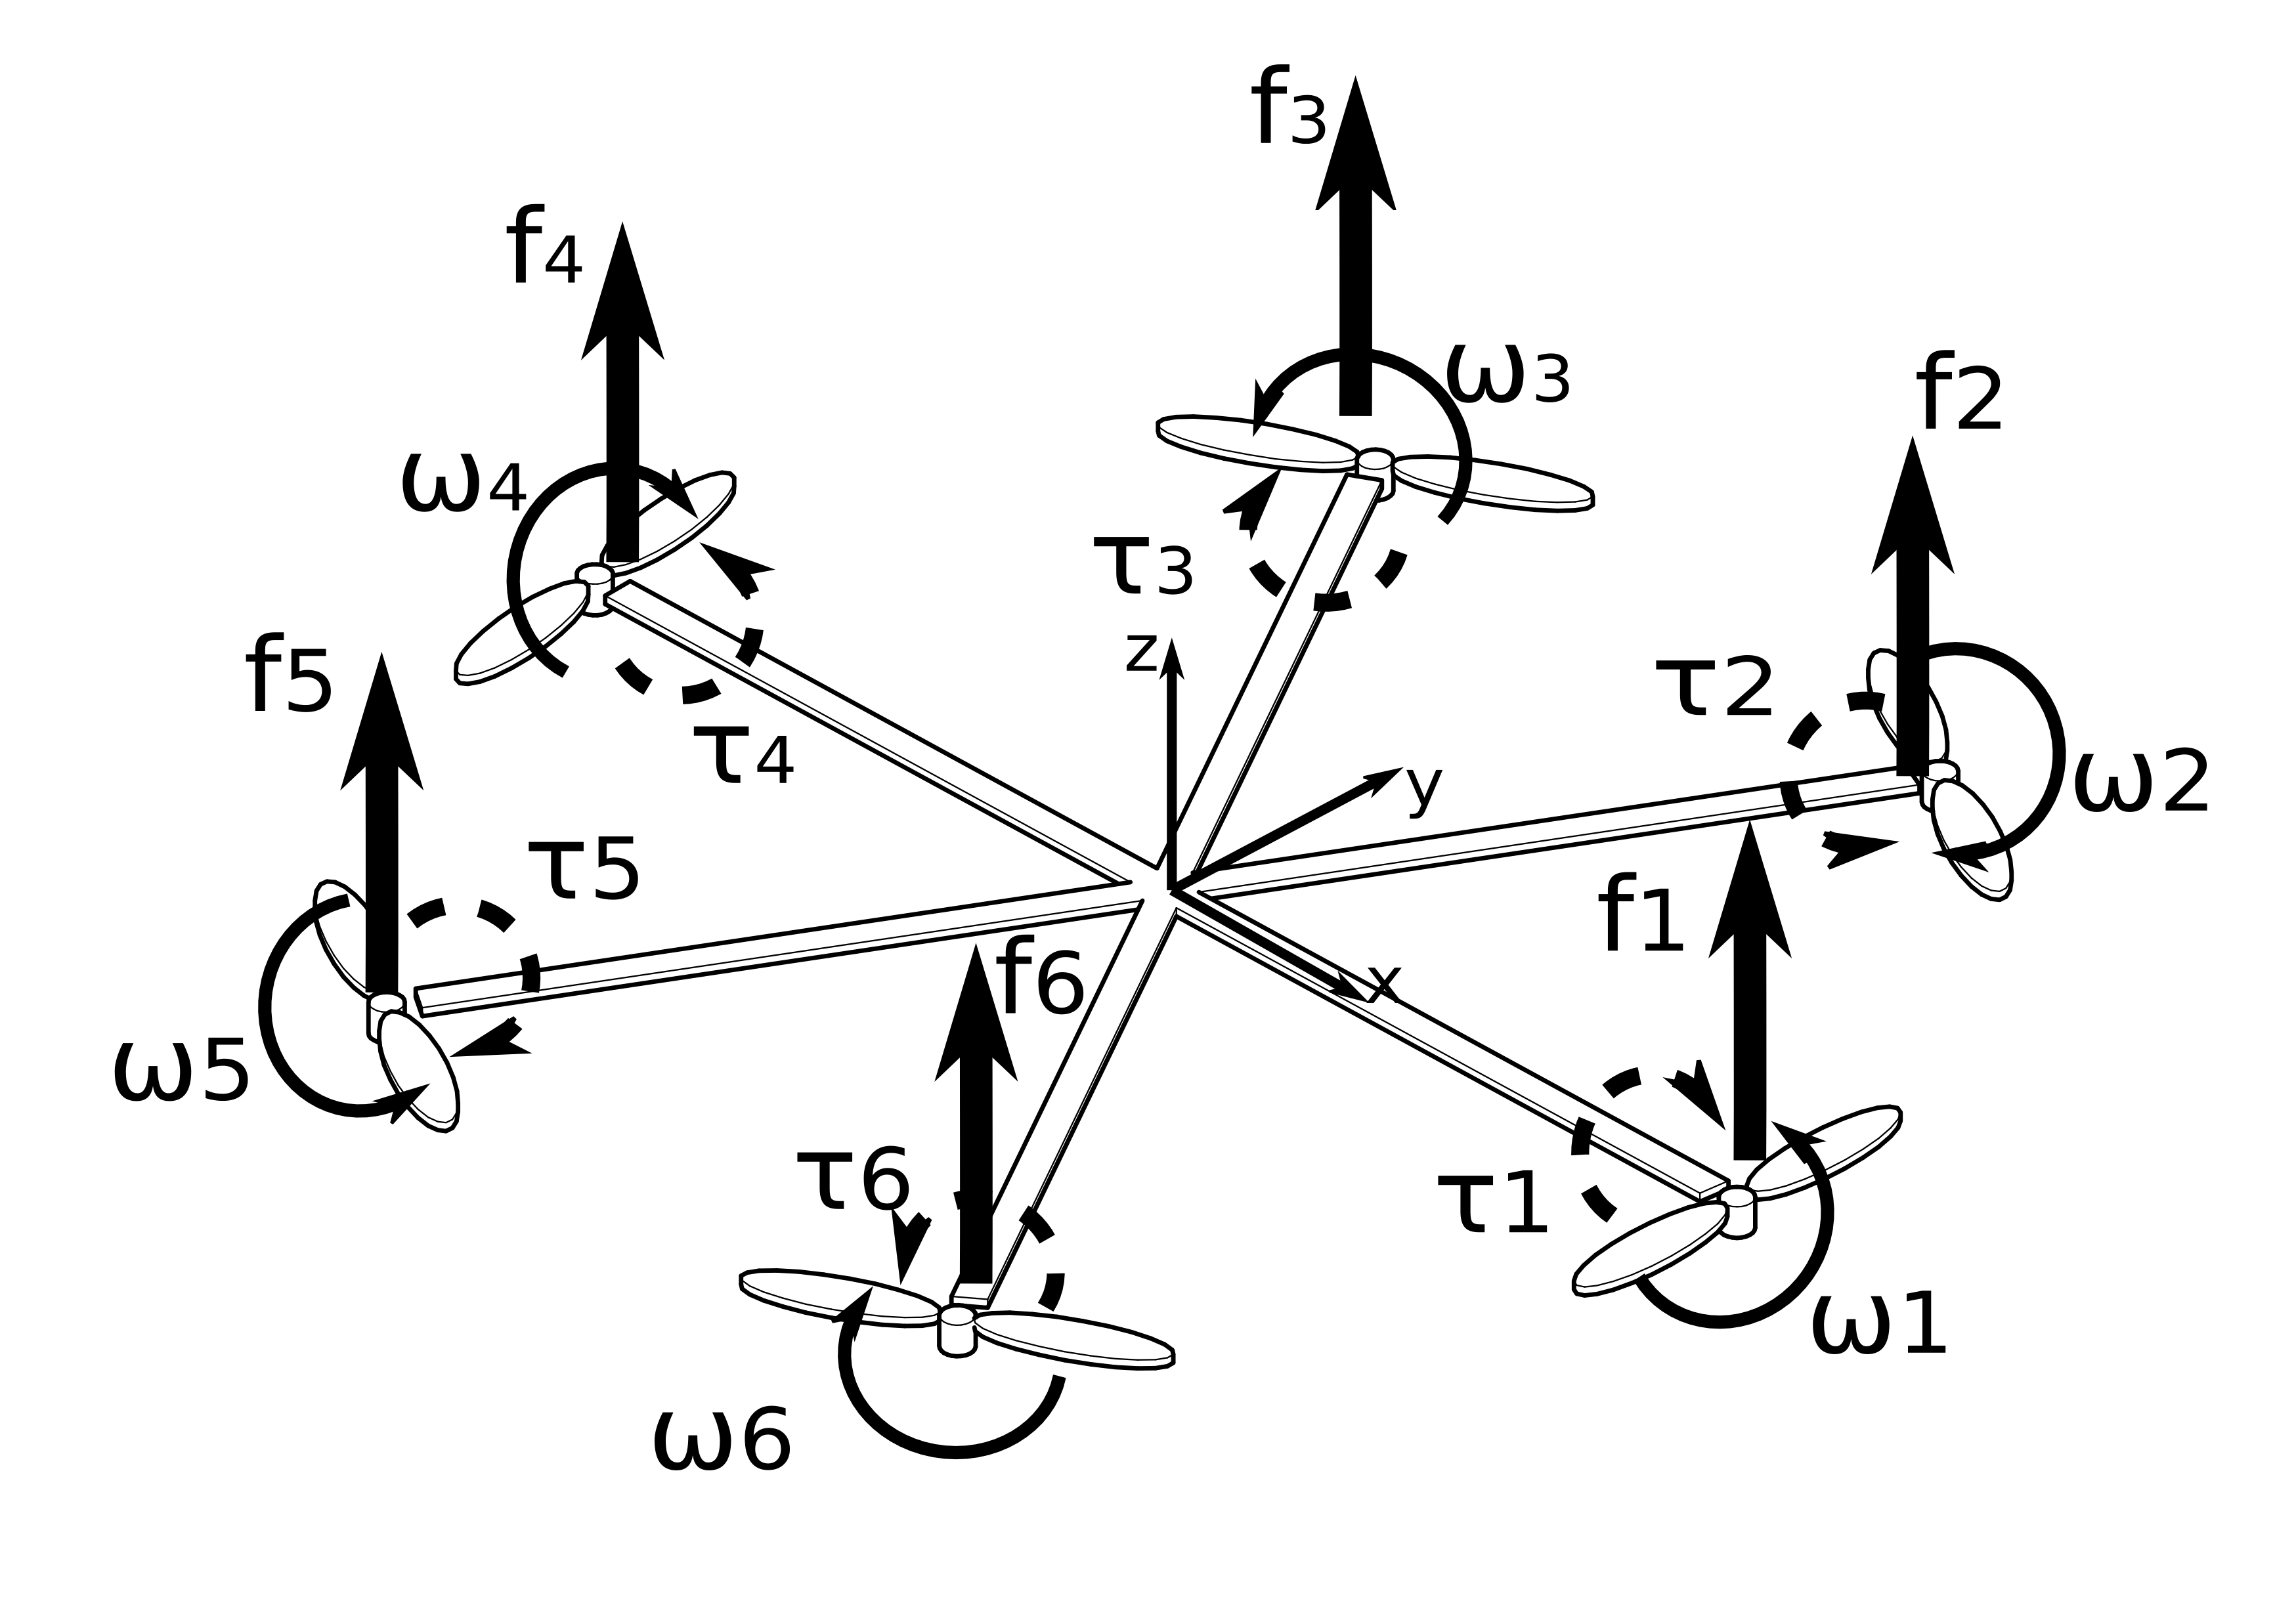
\includegraphics[width=8cm]{img/model_hexcopter.png}
\caption{Model hexkoptera\protect\footnotemark}
\label{fig:model}
\end{figure}
\footnotetext{Članak}
\subsection{Eulerovi kutovi}\label{sec:Euler}
Shematski prikaz hexkoptera prikazan je na slici~\ref{fig:model}. Da bi opisali gibanje hexkoptera potrebna su dva referentna sustava:\begin{itemize}
\item nepomični globalni koordinatni sustav,
\item pokretni lokalni koordinatni sustav hexkoptera.
\end{itemize}
Nultočka nepomičnog globalnog koordinatnog sustava postavljena je u jednoj točci (npr.~kut prostorije) te osi tog koordinatnog sustava su ortogonalne te raspoređene po \emph{desnoj orijentaciji} koordinatnog sustava u kojem je apsolutna linearna pozicija izražena kao $(\mathbf{x,y,z})$. Za određivanje orijentacije letjelice potrebno je definirati pokretni koordinatni sustava $(X_p,Y_p,Z_p)$ koji se giba zajedno s hexkoptera, a centar tog koordinatnog sustava nalazi se u centru mase hexkoptera i orijentirani je kao na slici~\ref{fig:model}. Smjer ortonormiranih vektora $X_p,Y_p,Z_p$ u svakom se trenutku može izraziti u odnosu prema nepomičnom globalnom koordinatnom sustavu. Slijed rotacija oko ortonormalnih vektora pomičnog koordinatnog sustava predstavljen je tzv.~Eulerovim kutovima --- skretanje \engl{roll} $\phi$, poniranje \engl{pitch} $\theta$ i valjanje \engl{yaw} $\psi$. Radi jednostavnosti označimo pokretni vektor pozicije i Eulerove kutove s $\xi = [x ~y ~z]^T$ i $\eta = [\phi ~\theta ~\psi]^T$. Transformaciju iz  lokalnog u globalni koordinatni sustav realizirana je s dobro znanom matricom rotacije \textbf{R} (izraz \ref{eq:matRot}) koja je ortogonalna.
\begin{equation}
	\begin{bmatrix}
	\cos\theta\cos\psi & \cos\psi\sin\theta\sin\phi-\cos\phi\sin\psi & \cos\phi\cos\psi\sin\theta+\sin\phi\sin\psi \\
	\cos\theta\sin\psi & \cos\phi\sin\psi+\sin\theta\sin\phi\sin\psi & \cos\phi\sin\theta\sin\psi-\cos\psi\sin\phi \\
	-\sin\theta & \cos\theta\sin\phi & \cos\theta\cos\phi \\
	\end{bmatrix}
	\label{eq:matRot}
\end{equation}
Kao posljedica, transformacijska matrica iz globalnog u lokalni koordinatni sustav je $\mathbf{R^{-1} = R^{T}}$. Matrica transformacije kutnih brzina iz lokalnog u globalni sustav je prikazana izrazom~\ref{eq:matBrzina}\footnote{Napomena: $\sec x = \frac{1}{\cos x}$}:
\begin{equation}
	\mathbf{W^{-1}_\eta} =
	\begin{bmatrix}
	1 & \sin\phi\tan\theta & \cos\phi\tan\theta \\
	0 & \cos\phi & -\sin\phi \\
	0 & \sec\theta\sin\phi & \cos\phi\sec\theta \\
	\end{bmatrix}
	\label{eq:matBrzina}
\end{equation}
Tada su zakoni transformacije~\ref{eq:v} i~\ref{eq:eta} gdje je $\nu$ definiran kao vektor $\nu=[\mathbf{p ~q ~r}]^T$.
\begin{align}
\nu&=\mathbf{W_\eta}\dot{\eta},\label{eq:v}\\
\dot{\eta}&=\mathbf{W^{-1}_\eta}\nu.\label{eq:eta}
\end{align}
Važno je uočiti da se $\mathbf{W^{-1}_\eta}$ može definirati samo i samo ako $\theta \neq \pi/2+k\pi, (k \in Z)$. Ovaj efekt kod Eulerovih formula je ograničenje, tipična situacija kad se gubi stupanj slobode. Uzimanjem drugačijeg prikaza orijentacije u prostoru identificiranog s četiri parametra, poznatijim kao kvaternioni čija generalna struktura je objašnjena u poglavlju~\ref{sec:Kvaternioni}. Prednost kvarteniona ne leži samo u nepostojanju singulariteta nego i kod jednostavnosti izračuna, što će biti kasnije objašnjeno.

\subsection{Kvaternioni}\label{sec:Kvaternioni}
U poglavlju~\ref{sec:Euler} može se primijetiti da bi rotacija krutog tijela u prostoru mogla biti predstavljena preko Eulerovih kutova, međutim zbog singularnosti transformacijskih zakona potrebno je koristiti novu parametrizaciju kvaternionima. Kvaternioni se obično koriste u razvoju računalnih igara i u 3D virtualnom svijetu, ali također i kao metoda za pozicioniranje krutog tijela u trodimenzionalnom prostoru. Kvaternioni se temelje na Eulerovom teoremu rotacije koji definira da svaki pomak krutog tijela gdje točka ostaje nepromijenjena je ekvivalentna rotaciji. Dakle, ako je $\alpha$ kut rotacije oko jediničnog vektora $\mathbf{u} = (u_1, ~u_2, ~u_3)$, moguće je definirati kvaternion $\mathbf{q} = [q_0 ~q_1 ~q_2 ~q_3]^T$, gdje su $q_0 = \cos(\alpha/2), ~q_1 = \sin(\alpha/2)u_1, ~q_2 = \sin(\alpha/2)u_2, ~q_3 = \sin(\alpha/2)u_3$, koji definira tri dimenzije rotacije. Kvaternioni uvijek moraju zadovoljavati jednadžbu ograničenosti (\ref{eq:normalniUvjet}) koja se zove normalni uvjet. 
\begin{align}
q^2_0+q^2_1+q^2_2+q^2_3=1 \label{eq:normalniUvjet}
\end{align}
Za razliku od Eulerovih kutova kvartenionske rotacije ne zahtijevaju skup unaprijed definiranih rotacijskih osi jer jedna os  se konstantno može mijenjati. Zbog svojstva ove metode da orijentacija ima samo jednu os rotacije, stupanj slobode se ne može izgubiti, odnosno ne postoji ograničenje. Transformacija translacijskih brzina gledano iz globalnog sustava može se izraziti preko \ref{eq:transBrzina} gdje je $\mathbf{Q}$ matrica~\ref{eq:matQ}.
\begin{align}
\xi=\mathbf{Q\xi_B} \label{eq:transBrzina}
\end{align}
\begin{equation}
	\mathbf{Q} =
	\begin{bmatrix}
	q^2_0+q^2_1-q^2_2-q^2_3 & 2(q_1q_2-q_0q_3) & 2(q_0q_2+q_1q_3) \\
	2(q_1q_2+q_0q_3) & q^2_0-q^2_1+q^2_2-q^2_3 & 2(q_2q_3-q_0q_1) \\
	2(q_1q_3-q_0q_2) & 2(q_0q_1+q_2q_3) & q^2_0-q^2_1-q^2_2+q^2_3 \\
	\end{bmatrix}
	\label{eq:matQ}
\end{equation}
Kao matrica $\mathbf{R}$ i matrica $\mathbf{Q}$ je ortogonalna, pa vrijedi također $\mathbf{Q^{-1} = Q^{T}}$. Kao kutna brzina, uključujući transformaciju može se izraziti kao $\mathbf{\dot{q}}=\mathbf{S}~\nu$ gdje matrica $\mathbf{S}$ ovisi o kvartenijskim komponentama prikazanim~\ref{eq:matS}.
\begin{equation}
	\mathbf{S} = \frac{1}{2}
	\begin{bmatrix}
	-q_1 & -q_2 & -q_3 \\
	q_0 & -q_3 & q_2 \\
	q_3 & q_0 & -q_1 \\
	-q_2 & q_1 & q_0 \\
	\end{bmatrix}
	\label{eq:matS}
\end{equation}
Zaključak, korist korištenjem kvaterniona je dvostruka: \begin{enumerate}
\item dohvaćanje svih pozicija (i onih kritičnih),
\item zahvaljujući linearnosti koeficijenata transformacijske matrice, izračun putem kvaterniona je učinkovitiji i stabilniji u odnosu s tradicionalnim izračunom.
\end{enumerate}

\subsection{Matematički model hexkoptera}
U ovom odjeljku prikazan je matematički model hexkoptera. Dinamika šest električnih motora je relativno brza pa će se stoga zanemariti. Cilj je odrediti matematičke jednadžbe koje opisuju dinamičko ponašanje hexkoptera pomoću generalizacije opisane sa slikom~\ref{fig:model} i poglavljem~\ref{sec:SimulacijskiDio}. Mogu se primijeniti Newton-Euler i Euler-Lagrange jednadžbe.\\

\subsubsection{Newton-Euler jednadžbe}
Gibanje krutog tijela može se razložiti na translacijsku i rotacijsku komponentu. Stoga, kako bi se opisala dinamika hexkoptera, pretpostavka je da je letjelica kruto tijelo pa se za izračun koriste Newton-Eulerove jednadžbe koje reguliraju linearno i kutno kretanje. Sila koja djeluje na hexkopter prikazana je \ref{eq:Sila}, gdje se pretpostavlja da je $m$ konstantna masa.
\begin{align}
\mathbf{F}&=\mathbf{\frac{d(m~v_B)}{dt}+\nu\times (m~v_b)} \label{eq:Sila}
\end{align}
Svaki rotor $i$ ima kutnu brzinu $\omega_i$ koja stvara silu $\mathbf{f_i}=k[0 ~0 ~\omega^2_i]$, gdje je $k$ konstanta potiska, dakle ukupan potisak \engl{thrust} $\mathbf{T_B}$ dan je s \ref{eq:TB} i \ref{eq:Tsila}
\begin{align}
\centering
\mathbf{T_B}&=\mathbf{[0 ~0 ~T]^T} \label{eq:TB} \\
\mathbf{T}&=\sum_{i=1}^{6}f_i=k\sum_{i=1}^{6}\omega_i \label{eq:Tsila}
\end{align}
Ukupan potisak zajedno s gravitacijom predstavlja ukupnu silu (izraz \ref{eq:Fukupna}) djelovanja na hexkopter.
\begin{align}
\mathbf{F}&=\mathbf{Q^TF_g+T_B} \label{eq:Fukupna}
\end{align}
Kao posljedica translacijska komponenta gibanja u lokalnom sustavu je \ref{eq:Flokalni}.
\begin{align}
m~\mathbf{\dot{v_B}+\nu\times (m~v_b)}&=\mathbf{Q^TF_g+T_B} \label{eq:Flokalni}
\end{align}
Da bi dobili istu jednadžbu u globalnom sustavu, potrebno je primijetiti da je centrifugalna sila poništena jer se globalni sustav ne rotira pa tako prethodna jednadžba postaje~\ref{eq:Flokalni}
\begin{align}
m~\mathbf{\ddot{\xi}}&=\mathbf{F_g+Q~T_B} \label{eq:Flokalni}
\end{align}
Nadalje, neka je $\mathbf{I}$ matrica inercija. Hexkopter ima simetričnu strukturu s obzirom na $X_b$-os, $Y_b$-os i $Z_b$-os, stoga je matrica inercija jedinična $\mathbf{I}=diag(\mathbf{I_{xx}, I_{yy}, I_{zz}})$. Kako ukupni vanjski moment $\mathbf{M}$ djeluje, uzimajući u obzir brzinu promjene kutnog momenta  $\mathbf{H=I\nu}$ tada je moment koji djeluje na hexkopter izražen s~\ref{eq:MomentHex}.
\begin{align}
\mathbf{M}&=\mathbf{\frac{d(I~\nu)}{dt}+\nu\times(I~\nu)} \label{eq:MomentHex}
\end{align}
Kutna brzina i akceleracija rotora stvaraju okretni moment prikazan \ref{eq:Torque} oko osi rotora, gdje je $b$ konstanta otpora tereta te gdje je $I_{M_i}$ moment inercije rotora $i$.
\begin{align}
\tau_{M_i}&=b~\omega^2_i+I_{M_i}~\dot{\omega_i} \label{eq:Torque}
\end{align}
Iz geometrijske strukture hexkoptera i od komponenata $\mathbf{f_i}$ i $\mathbf{\tau_{M_i}}$ u lokalnom koordinatnom sustavu moguće je dobiti informaciju o momentima \emph{roll, pitch i yaw} preko~\ref{eq:matTau}.
\begin{equation}
	\begin{bmatrix}
	\tau_{\phi} \\
	\tau_{\theta} \\
	\tau_{\psi}
	\end{bmatrix}
	=
	\begin{bmatrix}
	\frac{3}{4}kl(\omega^2_2+\omega^2_3-\omega^5_2-\omega^2_6) \\
	kl(-\omega^2_1-\frac{\omega^2_2}{4}+\frac{\omega^2_3}{4}+\omega^2_4+\frac{\omega^2_5}{4}-\frac{\omega^2_6}{4}) \\
	b(-\omega^2_1+\omega^2_2-\omega^2_3+\omega^2_4-\omega^2_5+\omega^2_6)+I_M(\dot{\omega^2_1}+\dot{\omega^2_2}+\dot{\omega^2_3}+\dot{\omega^2_4}+\dot{\omega^2_5}+\dot{\omega^2_6})
	\end{bmatrix}
	\label{eq:matTau}
\end{equation}
Ovdje je $l$ udaljenost između rotora i središta mase hexkoptera, a $\dot{x}\omega_i$ predstavlja vremensku derivaciju $\omega_i(t)$\footnote{Vremenska derivacija: $\frac{d\omega_i(t)}{dt}$}. Nadalje, jednadžba koja određuje dinamiku rotacije može se zapisati kao \ref{eq:rotDin} gdje $\mathbf{\Gamma}$ predstavlja žiroskopske sile i $\mathbf{\tau_B}$ vanjski okretni moment.
\begin{align}
\mathbf{I~\dot{\nu}+\nu\times(I~\nu)}+\Gamma&=\mathbf{\tau_B} \label{eq:rotDin}
\end{align}
Nakon kratkog izračuna dobije se \ref{eq:vDot} u kojoj je $\omega_{\Gamma}=\omega_1-\omega_2+\omega_3-\omega_4+\omega_5-\omega_6$.
\begin{equation}
	\dot{\nu} = \mathbf{I^{-1}} \Bigg(
	\begin{bmatrix}
	p \\
	q \\
	r
	\end{bmatrix}
	\times
	\begin{bmatrix}
	I_xx~p \\
	I_yy~q \\
	I_zz~r
	\end{bmatrix}
	-\mathbf{I_r}
	\begin{bmatrix}
	p \\
	q \\
	r
	\end{bmatrix}
	\times
	\begin{bmatrix}
	0 \\
	0 \\
	1
	\end{bmatrix}
	\mathbf{\omega_{\Gamma}}+\tau
	\Bigg)
	\label{eq:vDot}
\end{equation}
Inaće jednadžba \ref{eq:vDot} može se pisati kao \ref{eq:vDot2}
\begin{equation}
	\begin{bmatrix}
	\dot{p} \\
	\dot{q} \\
	\dot{r}
	\end{bmatrix}
	=
	\begin{bmatrix}
	(I_{yy}-I_{zz})~q~r/I_{xx} \\
	(I_{zz}-I_{xx})~p~r/I_{yy} \\
	(I_{xx}-I_{yy})~p~q/I_{zz}
	\end{bmatrix}
	-\mathbf{I_r}
	\begin{bmatrix}
	q/I_{xx} \\
	-p/I_{yy} \\
	0
	\end{bmatrix}
	\mathbf{\omega_{\Gamma}}+
	\begin{bmatrix}
	\tau_{\phi}/I_{xx} \\
	\tau_{\theta}/I_{yy} \\
	\tau_{\psi}/I_{zz}
	\end{bmatrix}
	\label{eq:vDot2}
\end{equation}
Konačno, nakon određivanja kutne brzine lako se odredi i kutno ubrzanje u globalnom koordinatnom sustavu preko izraza \ref{eq:angularAcceleration}.
\begin{align}
\mathbf{\ddot{q}}&=\mathbf{\frac{d(S~\nu)}{dt}} \label{eq:angularAcceleration}
\end{align}

\subsubsection{Euler-Lagrange jednadžbe}
Newton-Eulerova forma se temelji na ravnoteži sile i momenata. Alternativa tim jednadžbama, koristeći pristup temeljen na sačuvanje energije, su Euler-Lagrangeove jednadžbe. Prije svega, definicija Lagrangiana je izražena \ref{eq:Lagrangian} gdje je $E_t = (m/2)\mathbf{\dot{\xi}^T\dot{\xi}}$ translacijska kinetička energija, $E_r = (1/2)\mathbf{\nu^T~I~\nu}$ je kutna energija te $E_p=m~g~z$ je potencijalna energija gdje je $z$ visina hexkoptera.
\begin{align}
\mathcal{L}&=E_t+E_r-E_p \label{eq:Lagrangian}
\end{align}
Dinamički model letjelice dobiva se iz \ref{eq:dinModL} gdje $\bf f$ predstavlja vanjske sile koje utječu na potisak $\bf T_B$, $\tau=4\bf {S \tau_B}$ je generalizirani okretni moment i $\mathbf{w=\left[ \xi^T, q^T \right]}$ su Lagrangianove koordinate.
\begin{equation}
{d\over dt}\left({\partial {\cal L}\over \partial\dot{{\bf w}}}\right)-{\partial {\cal L}\over \partial{\bf w}}= \begin{bmatrix}\bf f \\ \bf\tau \end{bmatrix} \label{eq:dinModL}
\end{equation}
Budući da kinetička energija ne sadrži kombinaciju $\dot{\xi}$ i $\dot{\bf q}$, translacijska i rotacijska dinamika se mogu razmatrati zasebno. Translacijsko gibanje može se izraziti jednadžbom \ref{eq:transGiba} koja je jednaka kao \ref{eq:Flokalni}.
\begin{equation}
m\ddot{{\ \xi}}-{\bf F}_{g}={\bf f}={\bf Q\ T}_{B} \label{eq:transGiba}
\end{equation}
Potrebno je da se definira rotacijsko gibanje s generaliziranim koordinatama, ovdje brzina $\xi$ mora biti opisana kvaternionom $\bf q$.\\
Vidljivo je da se $\xi$ ne može dobiti iz \ref{eq:transBrzina} direktno, jer matrica $\bf S$ nije kvadratna, pa nije ni invertibilna. No produkt između $\bf S$ i njegove transponirane matrice je \ref{eq:productSt_S} gdje je $\cal I$ jedinična matrica dimenzije $3\times3$. 
\begin{equation}
{\bf S}^{T}{\bf S}={1\over 4}{\cal I} \label{eq:productSt_S}
\end{equation}
Dakle, lijevim množenjem s $\mathbf{S_T}$ izraza \ref{eq:productSt_S} dolazi se do \ref{eq:lijevoMnozenje} iz kojeg se dobije brzina \ref{eq:brzinaL}.
\begin{align}
{\bf S}^{T}\dot{{\bf q}}&={\bf S}^{T}{\bf S}{\ \nu}={1\over 4}{\cal I}{\ \nu} \label{eq:lijevoMnozenje} \\
{\ \nu}&=4{\bf S}^{T}\dot{{\bf q}} \label{eq:brzinaL}
\end{align}
Definiranjem \ref{eq:defJ}, kutna energija može se izraziti s \ref{eq:kutnaE}.
\begin{align}
{\bf J}&={\bf S\ I} \ {\bf S}^{T} \label{eq:defJ} \\
E_{r}&={1\over 2}{\ \nu}^{T}{\bf I}{\ \nu}=8\dot{{\ q}}^{T}{\bf J}\dot{{\ q}} \label{eq:kutnaE}
\end{align}
Sada je moguće napisati rotacijsku jednadžbu (\ref{eq:rotJedna}) preko kvaterniona $\bf q$. 
\begin{align}
8\bigg[2{\bf J}\ddot{{\bf q}}+2{d{\bf J}\over dt}\dot{q}-{\partial\over \partial {\bf q}}(\dot{q}^{T}{\bf J}\dot{q})\bigg]&={\ \tau} \label{eq:rotJedna}
\end{align}
Stoga je matematički model koji opisuje hexkopter izražen Euler-Lagrange formom prikazan \ref{eq:matModelL}.
\begin{align}
\ddot{{\bf q}}&={1\over 2}{\bf J}^{-1}\bigg[{1\over 8}{ \tau}-2{d{\bf J}\over dt}\dot{{\ q}}+{\partial\over \partial_{{\bf q}}}(\dot{q}^{T}{\bf J}\dot{q})\bigg] \label{eq:matModelL}
\end{align}
Može se uočiti da su ovi izrazi ekvivalentni izrazima \ref{eq:vDot} i \ref{eq:angularAcceleration}.

\subsection{Sinteza sustava upravljanja}
U ovom poglavlju projektira se regulator za slijeđenje željene trajektorije. Koriste se kvaternioni jer smanjuju nestabilnost te ubrzavaju numerički račun. Jednostavan i lako izvediv način upravljana, tj. njegove stabilizacije, realiziran je proporcionalno-derivacijskim (PD) regulatorom. PD regulatoru dodaje se integralna komponenta s ciljem smanjenja efekta fluktuacije \engl{fluctuations} hexkoptera koje su uzrokovane vanjskim poremećajima.
U izrazu \ref{eq:matQ} prikazana je kontrola leta hexkoptera. Konkretno, razvijena je jednostavna heuristička metoda za slijeđenje željene trajektorije. \\
Generalno, PID regulator koji prati referencu ima formu \ref{eq:PIDe} i \ref{eq:PIDu} gdje je $u(t)$ upravljački ulaz i $e(t)$ predstavlja pogrešku između reference $r_d(t)$ i trenutne pozicije $x(t)$.
\begin{align}
e(t) &= x_d(t) - x(t) \label{eq:PIDe} \\
u(t) &= K_p~e(t) + K_I \int_0^t {\mathrm{e(s)}\,\mathrm{d}s} + K_D {d\over dt} e(t) \label{eq:PIDu}
\end{align}
Koeficijenti $K_p, K_I, K_D$ predstavljaju parametre za proporcionalni, integracijski te derivacijski član PID regulatora. PID regulator se primjenjuje na sustav, prikazan \ref{eq:Torque} i \ref{eq:rotDin}, koji opisuje kretanje letjelice, tj.~njezin položaj. Može se pisati:
\begin{align}
d_x &= K_{x,P}~(x_d-x)+K_{x,D}~(\dot{x}_d-\dot{x})+K_{x,I} \int_0^t {\mathrm{(x_d-x)}\,\mathrm{d}s} \label{eq:PIDdy} \\
d_y &= K_{y,P}~(y_d-y)+K_{y,D}~(\dot{y}_d-\dot{y})+K_{y,I} \int_0^t {\mathrm{(y_d-y)}\,\mathrm{d}s} \label{eq:PIDdy} \\
d_z &= K_{z,P}~(z_d-z)+K_{z,D}~(\dot{z}_d-\dot{z})+K_{z,I} \int_0^t {\mathrm{(z_d-z)}\,\mathrm{d}s} \label{eq:PIDdy}
\end{align}
Razlika između klasičnih pristupa linearizacije, poput Lyapunove linearizacije ili linearizacije najmanjim kvadratima, i pristupa putem kvaterniona je u kvaternionskoj pogrešci $q_e$ --- ona je definirana kao razlika između željene orijentacije i trenutne izraženih preko kvaterniona. To dovodi do izraza \ref{eq:PIDqe1}-\ref{eq:PIDqe4} gdje je $\bf q_d$ kvaternion koji odgovara željenoj \emph{yaw} orijentaciji te kvaternion $\bf q$ koji odgovara trenutnoj orijentaciji. 
\begin{align}
q_{e,1} &= -q_{d,0}q_1 -q_{d,3}q_2 + q_{d,2}q_3 + q_{d,1}q_0 \label{eq:PIDqe1} \\
q_{e,2} &= q_{d,3}q_1 -q_{d,0}q_2 - q_{d,1}q_3 + q_{d,2}q_0 \label{eq:PIDqe2} \\
q_{e,3} &= -q_{d,2}q_1 +q_{d,1}q_2 - q_{d,0}q_3 + q_{d,3}q_0 \label{eq:PIDqe3} \\
q_{e,4} &= q_{d,1}q_1 +q_{d,2}q_2 + q_{d,3}q_3 + q_{d,0}q_0 \label{eq:PIDqe4}
\end{align}
Tada se komponente momenta $\tau_{\phi}, \tau_{\theta},\tau_{\psi}$ mogu se zapisati kao \ref{eq:tauPhi}-\ref{eq:tauPsi}.
\begin{align}
\tau_{\phi} &= (K_{\phi,D}~p + K_{\phi,P}~q_{e,1}~q_{e,4})~I_{xx} \label{eq:tauPhi} \\
\tau_{\theta} &= (K_{\theta,D}~q + 2K_{\theta,P}~q_{e,2}~q_{e,4})~I_{yy} \label{eq:tauTheta} \\
\tau_{\psi} &= (K_{\psi,D}~r + 2K_{\psi,P}~q_{e,3}~q_{e,4})~I_{zz} \label{eq:tauPsi}
\end{align}
Točne kutne brzine rotora $\omega_i$, koje su također upravljački ulazi izvedene su izrazima \ref{eq:omega1}-\ref{eq:omega6} gdje $k$ označuje potisnu konstantu, $b$ označuje vučnu konstantu, a $l$ predstavlja udaljenost između rotora i centra mase hexkoptera.
\begin{align}
\omega^2_1 &= \frac{T}{6k} - \frac{2\tau_{\theta}}{5kl} - \frac{\tau_{\psi}}{10b} \label{eq:omega1} \\
\omega^2_2 &= \frac{T}{6k} + \frac{\tau_{\phi}}{3kl} -\frac{2\tau_{\theta}}{5kl} + \frac{\tau_{\psi}}{5b} \label{eq:omega2} \\
\omega^2_3 &= \frac{T}{6k} + \frac{\tau_{\phi}}{3kl} + \frac{2\tau_{\theta}}{5kl} - \frac{\tau_{\psi}}{5b} \label{eq:omega3} \\
\omega^2_4 &= \frac{T}{6k} + \frac{2\tau_{\theta}}{5kl} + \frac{\tau_{\psi}}{10b} \label{eq:omega4} \\
\omega^2_5 &= \frac{T}{6k} - \frac{\tau_{\phi}}{3kl} + \frac{2\tau_{\theta}}{5kl} - \frac{\tau_{\psi}}{5b} \label{eq:omega5} \\
\omega^2_6 &= \frac{T}{6k} - \frac{\tau_{\phi}}{3kl} -\frac{2\tau_{\theta}}{5kl} + \frac{\tau_{\psi}}{5b} \label{eq:omega6} 
\end{align}
Neka $\bf \ddot{\xi}, \dot{\xi}$ i $\bf q_3$ definiraju željenu trajektoriju. Koristeći izraze \ref{eq:Flokalni}-\ref{eq:vDot} i normalni uvjet \ref{eq:normalniUvjet} možemo izraziti $q_0$ (\ref{eq:q0}), $q_1$ (\ref{eq:q1}), $q_2$ (\ref{eq:q2}) i ukupni potisak $\bf T$ (\ref{eq:T}). 
\begin{align}
q_0 &= \sqrt{\frac{1}{2} + \frac{d_z+g}{2\sqrt{d^2_x+d^2_y+(d_z+g)^2}}-q^2_3} \label{eq:q0} \\
T &= \frac{m(d_z + g)}{2~(q^2_0 + q^2_3)-1} \label{eq:T} \\
q_1 &= \frac{m(d_z q_3 - d_y q_0)}{(q^2_0 + q^2_3)~2T} \label{eq:q1} \\
q_2 &= \frac{m(d_z q_0 - d_y q_3)}{(q^2_0 + q^2_3)~2T} \label{eq:q2}
\end{align}
Valja se prisjetiti da se hexkopterom upravlja podešavanjem brzina vrtnje rotora koji se pokreću elektromotorima. 


\subsection{Matlab}

\section{Eksperimentalni dio}
Cijena modernih bespilotnih letjelica doseže nekoliko desetaka tisuća kuna (postoje i skuplje) koje imaju ugrađeno mnogo senzora. U našem eksperimentalnom dijelu koristena je jeftinija verzija koja nema toliko senzora, pa su zbog tog korišteni dodatni vizualni senzori koji određuju položaj letjelice u prostoru. 
\subsection{Postav}

\subsection{ROS kod}

\subsection{Rezultati}
 
\begin{table}[h!]
  \caption{Kratki slikovni prikaz osnovnih vrsta i oblika dronova\citep{vrsteDronova}}
  \label{tbl:vrsteDronova}
  \begin{center}
  	\begin{tabular}{ | c | c | c | }
    \hline
    Vrsta & Prednosti & Mane \\ \hline
    \begin{minipage}{.3\textwidth}
    	Quadcopter (letjelica s četiri elise)
      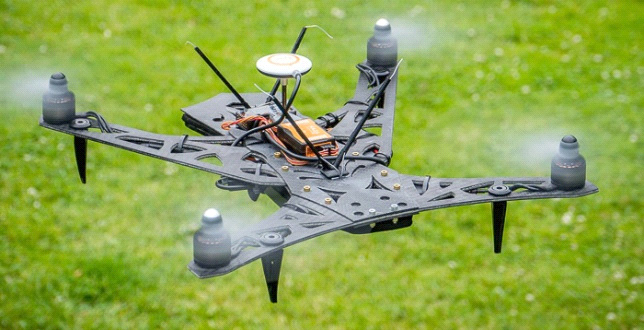
\includegraphics[width=\linewidth, height=25mm]{img/quadcopter.png}
    \end{minipage}
    &
    \begin{minipage}{5cm}
      \begin{itemize}
        \item može lebdjeti (stacionarni let)
        \item može poletjeti s mjesta i sletjeti
      \end{itemize}
    \end{minipage}
    & 
    \begin{minipage}{5cm}
      \begin{itemize}
        \item nije za velike udaljenosti ni visine
        \item kratak vijek trajanja baterije
      \end{itemize}
    \end{minipage}
    \\ \hline
    \begin{minipage}{.3\textwidth}
    	Oblik zrakoplova \engl{plane shaped drone}
      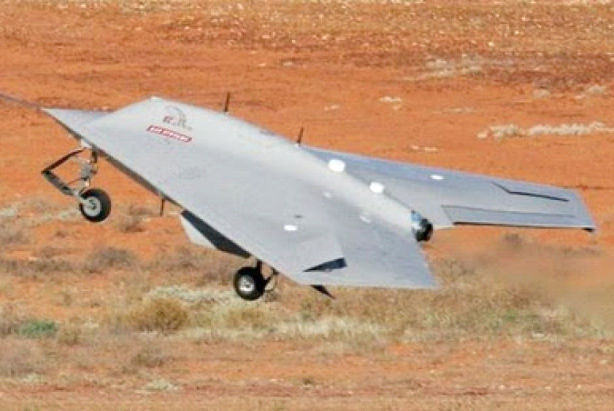
\includegraphics[width=\linewidth, height=25mm]{img/plane_shaped_drone.png}
    \end{minipage}
    &
    \begin{minipage}{5cm}
    	\begin{itemize}
      	\item dobar manevar
        \item velike udaljenosti
        \item velike visine
      	\end{itemize}
    \end{minipage}
    & 
    \begin{minipage}{5cm}
      \begin{itemize}
      	\item ne može lebdjeti (zasad)
      	\item ne može poletjeti s mjesta (zasad)
      \end{itemize}
    \end{minipage}
    \\ \hline
    \begin{minipage}{.3\textwidth}
      Oblik muhe \engl{insect fly shaped drone}
      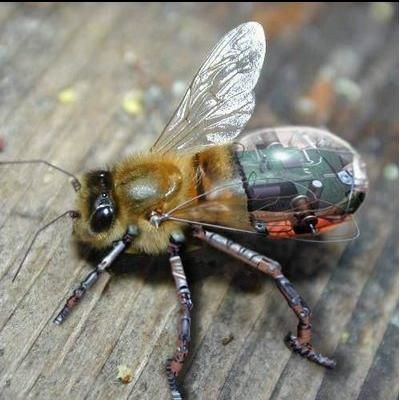
\includegraphics[width=\linewidth, height=25mm]{img/insect_fly_shaped_drone.png}
    \end{minipage}
    &
    \begin{minipage}{5cm}
      \begin{itemize}
        \item vrlo mali
        \item može se zavlačiti te ići na nepristupačan teren
        \item oponaša kretanje muhe ili insekta
      \end{itemize}
    \end{minipage}
    & 
    \begin{minipage}{5cm}
      \begin{itemize}
        \item mali dron = mala baterija
      \end{itemize}
    \end{minipage}
    \\ \hline
  	\end{tabular}
  \end{center}
\end{table}

\chapter{Proba}
Uvod rada. Nakon uvoda dolaze poglavlja u kojima se obrađuje tema.
\section{Odjeljak 1.1}
Tekst o odjeljku
\subsection{Pododjeljak}
\emph{How can we eat?}
Popis fusnota\footnote{Objašnjenja koja se prikazuju
na dnu stranice} nije potreban.
\section{Dodavanje posvete}
\label{sec:posveta}
Za navedeno pogledajte odjeljke \ref{sec:posveta}
\begin{itemize}
	\item prva stavka,
	\item druga stavka,
	\begin{enumerate}
		\item druga razina.
	\end{enumerate}
\end{itemize}

\begin{table}[htb]
\caption{Konstante}
\label{tbl:konstante}
\centering
\begin{tabular}{llr} \toprule
Konstanta & Opis & Vrijednost\\ \midrule
$\pi$ & Pi & 3.14159 \\
$e$ & Eulerov broj & 2.71828 \\
$\varphi$ & Zlatni rez & 1.61803 \\ \bottomrule
\end{tabular}
\end{table}

\begin{figure}[htb]
\centering

\includegraphics[width=5cm]{img/fer_logo.jpg}
\caption{Logo FER-a}
\label{fig:fer-logo}
\end{figure}

‘Prva dama: $\sin^2 \varphi + \cos^2 \varphi = 1$.’ \citep{ungar2002uvod} \cite{oetiket2007lshort}
\begin{align}
a&=b+c,\label{eq:a}\\
d&=e+f+g,\\
h&=i+j.\label{eq:h}
\end{align}

Dodatak dokumenta \engl{appendix}.

Primjer korištenja enumitem paketa dan je u \citep{collins2008enum}.
\citet{collins2008enum} opisuje korištenje enumitem paketa.
\cite{greenwade93}
Text ... citation: \cite{greenwade93}.

\chapter{Zaključak}
Zaključak.

\bibliographystyle{fer}
\bibliography{literatura}

\begin{sazetak}
Sažetak na hrvatskom jeziku.

\kljucnerijeci{Ključne riječi, odvojene zarezima.}
\end{sazetak}

% TODO: Navedite naslov na engleskom jeziku.
\engtitle{Title}
\begin{abstract}
Abstract.

\keywords{Keywords.}
\end{abstract}

\end{document}
